\documentclass{article}

% if you need to pass options to natbib, use, e.g.:
%     \PassOptionsToPackage{numbers, compress}{natbib}
% before loading neurips_2020
\PassOptionsToPackage{sort,numbers}{natbib}
% ready for submission
 \usepackage{neurips_2020}

% to compile a preprint version, e.g., for submission to arXiv, add add the
% [preprint] option:
 %    \usepackage[preprint]{neurips_2020}

% to compile a camera-ready version, add the [final] option, e.g.:
%     \usepackage[final]{neurips_2020}

% to avoid loading the natbib package, add option nonatbib:
     %\usepackage[nonatbib]{neurips_2020}

\usepackage[utf8]{inputenc} % allow utf-8 input
\usepackage[T1]{fontenc}    % use 8-bit T1 fonts
\usepackage{hyperref}       % hyperlinks
\usepackage{url}            % simple URL typesetting
\usepackage{booktabs}       % professional-quality tables
\usepackage{amsfonts}       % blackboard math symbols
\usepackage{nicefrac}       % compact symbols for 1/2, etc.
\usepackage{microtype}      % microtypography


\usepackage{graphicx}
\usepackage{subfig}
\usepackage{amsmath}



\title{Reflexive Reinforcement Learning}

% The \author macro works with any number of authors. There are two commands
% used to separate the names and addresses of multiple authors: \And and \AND.
%
% Using \And between authors leaves it to LaTeX to determine where to break the
% lines. Using \AND forces a line break at that point. So, if LaTeX puts 3 of 4
% authors names on the first line, and the last on the second line, try using
% \AND instead of \And before the third author name.

\author{
  B. I. Lyons \quad J. Michael Herrmann \\
  \\
  Institute for Perception, Action and Behaviour\\
  University of Edinburgh\\
  United Kingdom, EH8 9AB \\
  %\texttt{\{Billy.Lyons, Michael.Herrmann\}@ed.ac.uk} \\
}

\begin{document}

\maketitle

\begin{abstract}
We propose the method of reflexive reinforcement learning (RRL), an extension of self-motivated reinforcement learning that enables the generation of autonomous learning behaviours in the absence of explicit external rewards and where actions can be taken in order to obtain information about the environment. This framework includes entropy reduction of distribution over states, reward functions and actions, as well as integration of non-task-specific information such as the theory of empowerment. RRL is a tool with which an agent can use the current representation of the value, of its state, and of the environment to identify regions of a state space that are interesting through a variety of simple, and distinct reward schemes. We continue to show that RRL is naturally applicable in the multi-agent domain, where agents are shown to be able to identify socially valuable regions of the state space.%, 
%develop complementary behaviours or to partition the space into domains.
%
Finally, we discuss the Markov property in the context of RRL and the demonstrate the benefits of its integration with traditional reinforcement learning approaches.
\end{abstract}

\section{Introduction}

Intrinsic motivation~\cite{chentanez2005intrinsically} has been proposed in order to realise 
reinforcement learning (RL) in the absence of external rewards. It has been 
characterised~\cite{pathak2017curiosity} to follow either or both of two main goals:
\begin{itemize}
	\item Encouraging exploration of unseen or interesting states, such as states that
		are central or risky, represent momentous decisions, or are at the 
		boundary of a currently known domain;
	\item Reduction of uncertainty by improvement of the prediction of consequences of 
		actions or of the estimation of various probability distributions over
		states, actions and rewards.
\end{itemize}
These two goals may not be achievable at the same time, and various methods to negotiate the
goals have been studied in the context of autonomous learning and self-organisation 
of behaviour~\cite{bialek1999predictive,der2012playful,klyubin2005empowerment}.
%??? more references ???
It was shown that options or elementary behaviours can be created by these methods that can 
also be extended for the generation of self-organised plans~\cite{blaes2019control}. 
%what is wrong the IMRL ???

We are proposing a new view on intrinsic motivated RL (IMRL) which can summarised by the 
maxim: \emph{Act such that inverse reinforcement learning works well}. 
Inverse RL~\cite{ng2000algorithms} aims at the reconstruction of the reward distribution based
on the observed behaviour of a supposed RL agent and thus at the identification of reasons 
for its behaviour. In this way, we will refer to inverse RL not as a problem to be solved, 
but as an easily solvable problem to be posed: 
the self-motivated agent aims at generating a behaviour in its environment that 
is particularly clear with respect to underlying reasons given the specificity and 
stochasticity of the environment. 

The potential advantages of this approach are obvious: The
agent will tend to produce modes of behaviour that are both robust and informative, i.e.~it
will try to find a compromise to the mentioned dilemma of intrinsically motivated behaviour.
The intrinsically generated behaviour may be further modulated by later or intermittently 
available external rewards, but will be biased towards readily analysable and explainable
policies. 

In inverse RL the trivial solution of interpreting the observed behaviour as random 
needs to be avoided by an additional criterion such as maximal entropy~\cite{ziebart2008maximum}. 
In the same way, the trivial case of producing trivial behaviours in IMRL is avoided.
As there are many aspects to RL and inverse RL, a wide area of \emph{reflexive} RL (RRL) is 
conceivable that we will trace out by means of a few special cases.


%% to be updated ??? 
The rest of this paper is organised as follows: After discussion of prior relevant work, we specify the reinforcement learning problem that we are going to study here in 	Sect.~\ref{Methods}, where we also describe the theory underpinning the robotic implementation. Sect.~\ref{Methods} outlines the algorithm that we used, as well as a description of the experimental setup that was utilised. The results of the experiments are provided and analysed also in Sect.~\ref{Results}. The conclusions of the work and future work are given in Sect.~\ref{Discussion}.

%In the present case this means that if reasons for actions are discernible for an 
%observer or a different agent they
%will take into account a reflexive evaluation of the agent. 

\section{Background}

\subsection{Reinforcement Learning}

RL aims at finding solutions to the Bellman problem of reconstructing a value function that obeys
\begin{equation}
	V^*(s)=\max_a \left(R(s,a) + \gamma \sum_{s'} P(s'|s,a) V^*(s')\right)
\end{equation} 
in the case of deterministically chosen maximising actions in a Markovian decision problem, where
$s$ is the current and $s'$ the subsequent state, and action $a$ is executable in state $s$.
This includes two aspects: the maximisation of the utility over some time horizon and the 
identification and control of trajectories towards high-utility states. 

Classical RL algorithms
have focused mainly on the maximisation problem and did not provide theoretical 
solutions to the exploration problem, also many heuristic approaches exist.
%instead soft policies were designed, random state or parameter noise was induced or
%by either ignoring the problem such as in policy gradient methods or taking it as learnable 
Recently, and possibly inspired by the free-energy paradigm~\cite{friston2006free}
but essentially going back to Refs.~\cite{still2012information} and \cite{bialek1999predictive}, 
the RL problem has been considered in an information-theoretical 
formulation~\cite{tschantz2020reinforcement}, 
where information gain can be  systematically incorporated into the utility function

It remains open in this approach how to choose realistic global priors, how to avoid
local optima, and what metrics are to be used for the computationally 
demanding function approximation of probability distributions for policy, rewards, and 
state transitions, and how to resolve the relationship between information available 
in the state space and the utility, i.e.~the problem of how reward-related gains and 
information-related costs are cleared. The latter problem is solvable in general as
the tipping point of this balance depends on the environment and the representation thereof
in the algorithm~\cite{smith2018evaluation}, but with that the generality of the 
information-theoretic approach is limited.
%and how estimation errors interfere with the optimality of the policy.
%In addition it is to be asked whether the extraction of a 
%policy does require the estimation of high-dimensional probability distributions

%In intrinsically motivated RL any external rewards are initially assumed to be absent
%such that properties of the own body, sensorimotor contingencies, and the 
%environmental relationships can be explored

%We argue that once an intrinsic reward criterion is defined, there is no need for an 
%explicit representation beyond the orthogonal representation of value and policy.

%Experimentation can be defined as ``the process of trying methods, activities etc. to discover what effect they have''~\citep{walter2008cambridge}, and is an essential step in the acquisition of knowledge. This learning criterion implies that for effective learning of models, there is a dichotomy present, in which an agent must act to reduce the prediction error of the model it is generating, whilst also maximising the information gain it can obtain from the environment, that is to say, a learning agent must both learn to accurately perceive the effects of its actions on the environment, but must also aim to select actions with the intent of generating the most information.

%This dichotomy is another information centric representation of the \emph{exploration-exploitation dilemma}, and has attracted researchers from multiple disciplines following the publication of J.G. March in 1991~\citep{march1991exploration}, with greatly cited publications in neuroscience~\citep{laureiro2010neuroscientific}, marketing~\citep{prange2009role} and our own, computer science~\citep{sutton1999reinforcement}.

%In this paper we consider the need for reflexive exploration in learning tasks by maximising entropy. We propose that utilising a purely entropy maximisation approach is akin to empowerment~\citep{klyubin2005empowerment} over its action space, such that the agent continues to move to regions which value future freedom of movement, and attempt to find a balance between both goals to define new regions of interest. We continue by showing that this approach is highly flexible with simple rewards in both single agent and multi-agent environments to highlight key areas of a space, with a view to use this information for intrinsic motivation.

%Machine learning usually consists in the optimisation of a given cost function that is given in terms of the accumulated reward in reinforcement learning (RL). 
%In autonomous learning the cost function does usually not provide sufficient information for the agent to decide about actions and random action choices for exploration are inefficient.
%Therefore, the agent needs to produce incentives to act on its own based on intrinsic motivation.
%We here are interested in an agent that has no specific goal, or indeed, is unable to obtain any information related to the goal temporarily.  In such an instance that a robot is lost or unable to determine the goal, it should default to an intrinsic motivation to move to an area where it can learn or be suitably located to perform a task in the future, whilst still being adaptive to its environment.

%As such it is important to consider the value of a state in a way that is not tied directly to some desired goal, but instead considers the most \emph{interesting} state as one which is most valuable. Such approaches have been discussed as alternative to reinforcement leaning, for example, in  the theories of empowerment~\citep{klyubin2005empowerment} (see also Sect.~\ref{emp}), in homeokinesis~\citep{der2012playful} or in Friston's programme~\citep{friston2006free} to employ the free energy to the same goal, as well as some studies that have considered the self-referential aspect alongside traditional reinforcement learning methods~\citep{pathak2017curiosity}. All of these approaches have their own weaknesses which include, immense computational cost, limitation to low-level behaviours, or conceptual relation to the explanandum, at least some of which may be a necessary cost for the gain of autonomy of the agent that rely on the resp.~principle.


%For the current purpose it suffices to consider the basic reinforcement learning (RL) algorithm~\citep{sutton2018reinforcement}. 
%Given a finite Markov decision problem (MDP), $(X, x_0, A, R, P)$, where $X$ is a finite set of states with start state $x_0$, $A$ a finite set of actions, and $R$ is a function that assigns to each triplet (state, action and following state) a random variable $R$ which 
%provides a stochastic evaluation. The task is to maximise the expected, accumulative, discounted amount of this number which means to choose the actions such soon high values of $r$ are obtained.  
%This task can be easily achieved if a function $Q$ is known that contains the information about the expected reward, so that a large part of RL research is related to function approximation techniques.
%In this paper we use a traditional function approximation approach for state-action pairs
%\begin{eqnarray}
%Q^{\pi_w}(x,a)&=&E_{\pi_w}\left\lbrace \sum_{t=0}^\infty\gamma^{t} r_t| x_0 = x, a_0 = a \right\rbrace \\
%V^{\pi_w}(x)&=&E_{\pi_w}\left\lbrace \sum_{t=0}^\infty\gamma^{t} r_t | x_0 = x \right\rbrace 
%\end{eqnarray}
%where \textbf{w} is updated by
%\begin{equation} \label{faeqn}
%\textbf{w} \leftarrow \textbf{w} + \alpha \left[r_t + \gamma \hat{q}(x_{t+1},a_{t+1},\textbf{w}) -  \hat{q}(x,a,\textbf{w}) \right]
%\end{equation}
%where $\hat{q}(x_{t+1},a_{t+1})$ is an unbiased estimator of $q_{\pi}(x,a)$, and $r_t$ is the reward supplied to the agent, with step size $\alpha$, and learning rate $\gamma$.

For simplicity, we will stick here with the discrete case and discuss generalisations in the supplementary material.

\subsection{Inverse RL\label{invRL}}

In an RL problem with discrete actions $a \in \mathcal{A}$ we can try to recover 
the value function given action-conditioned state transitions $P^a(s',s)$~\cite{ng2000algorithms}
such that
\begin{equation}
	\sum_{s'} V\left(s'\right) P\left(s'|s,a) \right)
	\ge\sum_{s'} V\left(s'\right) P\left(s'|s,b\right)
	%\,\,\,\,\forall b\in{\cal A}\backslash\left\{ a\right\} 
	\label{inRLeq}
\end{equation}
for any $b \in \mathcal{A}$ different from $a$. If the reward depends only in the current state,
then the relation $R(s)=\left(I-\gamma P^{a}\right)V(s)$ can be used on order to reconstruct 
the structure of the reward distribution. Because $V\equiv 0$ (or $R\equiv 0$) is a trivial 
solution of Eq.~\ref{inRLeq},
additional conditions need to be imposed such as a maximal difference between optimal and second-best action~\cite{ng2000algorithms}  or, more generally, maximum entropy reward 
distribution~\cite{ziebart2008maximum} or adversarial schemes~\cite{pfau2016connecting}. 

Inverse RL presupposes that the observed agent is already well-trained, such that 
its behaviour expressed the rewards structure; however, continuing to generate data after
self-learning would not be meaningful in the present case. Additionally, the agent should not aim
at exploiting a partcular inverse RL algorithm. Therefore, the agent does not aim at actually 
solving the inverse RL problem, and we can assume various stages of inverse RL in order 
to enable autonomous behaviour in the agent. So the agent should set itself rewards that:
\begin{itemize}
	\item single out a particular state or that appear identical based on a given sensor configuration;
	\item have a spatial configuration and preproducibility to stick out the noise;
	\item single out states that are providing optimally controllable options;
	\item are compatible with a maximum entropy distribution of paths.
\end{itemize}
In order to make these points more clearly, we will discuss the concept of empowerment next.
%Conclusions from inverse RL: 

%Relation to homeokinesis???

\subsection{Discounted empowerment\label{emp}\label{gammares}}

The concept of \emph{empowerment}~\citep{klyubin2005empowerment} is a way to 
express the value of a state without consideration of goal-oriented behaviour.
It can be understood as a quantification of an agent's control over its environment
or, likewise, of the freedom of choice of actions and of the 
level of reproducibility of a sequence of actions~\citep{salge2014empowerment}.
The original aim  of this concept was not to motivate exploration, 
but instead to identify \emph{preferred} states in an environment that is already known.
If the agent is within the state $s_t$ the $n$-step empowerment is defined based on mutual 
information
\begin{equation}
\mathfrak{E}_{n}\left(s_{t}\right)=\max_{\pi:s\to a}\,{\cal I}\left(s_{t+n};a_{t+n-1},\dots,a_{t}\right)\label{eq:n_powerment}
\end{equation}
so that the task is to find a policy for which the mutual information between the next actions and the set of states is maximal.

%\subsubsection{Discounted Empowerment \label{gammares}}
Empowerment usually requires full prior information as well as the evaluation of all possible time series and states to determine which state or states are best for the agent to occupy over a given $n$-step time horizon. In this sense it is quite similar to POMDPs~\cite{kaelbling1998planning}, 
but without any external rewards, apart from the information gains.
%As such it requires prior knowledge of all state transition probabilities $p(s_{t+1}|s_t, a_t)$ for all $s_t, a_t$ and to be tested over all policies.
In the context of RL, this level of computational complexity appears unnecessary because the precise value of $\mathfrak{E}_{n}$ (\ref{eq:n_powerment}) is largely irrelevant, alternatively an approximation of the empowerment can be produced iteratively by considering the entropy gain per step 
$\mathfrak{E}_{1}\left(s_{t}\right)$ and then summing over the time
horizon specified by the RL discount factor $\gamma$.
\begin{equation}
	\mathfrak{E}_{\gamma}\left(s_{t}\right)=\sum_{t=t_0}^\infty
	\gamma^{t-t_0}\mathfrak{E}_{1}\left(s_{t}\right)
	\label{eq:gamma_powerment}
\end{equation}
The concept of $\gamma$-empowerment introduced in 
Eq.~\ref{eq:gamma_powerment} is similar in information provided, but not equivalent to the original 
concept (\ref{eq:n_powerment}), because it does not have a 
crisp time horizon and also because it allows for different 
measures of the local empowerment 
$\mathfrak{E}_{1}\left(s_{t}\right)$ as long as 
the tendency of the agent to roam without restrictions is captured in
an appropriate way, see Sect.~\ref{Actions_etc}.

\section{Reflexive Reinforcement Learning}
We propose \emph{reflexive reinforcement learning} (RRL) as a more general approach that combines self-generated rewards and manipulation of the
value function or policy in autonomous learning based on the additional principles:
\begin{itemize}
\item versatility and empowerment;
\item social interaction and emotional learning;
\item optimal internal representations;
\item optimal substructure.
\end{itemize}

We are interested in extracting knowledge from these values, which has been done
related to temporal fluctuations, but %it becomes more
is perhaps more interesting if spatial variations are considered, as, in this way information directly
related to the environment can be extracted, whereas temporal fluctuations mainly provide
information about the learning process~\citep{herrmann1995efficient}. We will consider, in addition, qualitative effects of actions and loops which can also be used to characterise the environment. These approaches will be considered in more details 
in the following subsections.
\cite{balakrishnan2019incorporating}

%\subsection{Reflexive Reinforcement Learning}
In the case of reflexive reinforcement learning the \emph{reflexive component} informs state valuation through standard reinforcement learning. This additional component allows that we are able to switch between a variety of different components for different needs, as we will show in Sect.~\ref{Results}.

\begin{figure}[ht] 
\centering
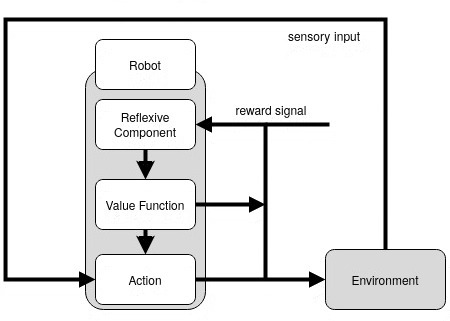
\includegraphics[scale=0.45]{pics/RRLfig.jpg} 
	\caption{Schematic representation of RRL.\label{rrlfig}}
\end{figure}

As seen in Fig.~\ref{rrlfig}, the reflexive component will receive external rewards from the environment through the observation of the state, and this adjusted reward is used to inform the state valuation or valuations. In this manner it is possible for the agent to continue to receive information pertinent to potential tasks as it maintains its motivation to explore the environment through the different valuations during periods of no task or when in a state where it is lost.
%The methods discussed in this paper are what we here call \emph{Reflexive Reinforcement Learning} (RRL) and each have in common that the reward in a reinforcement learning task refers reflexively to the values that are built by the algorithm based on the reward. This is problematic but interesting for autonomous learning, as the agent can use its own learning progress as a source of information. There are three conditions that need to be observed:
%\begin{itemize}
%	\item[$\bullet$] The information accumulated should be meaningful, i.e.~the agent used the
%		time when no goal or target behaviour is to be followed for the 
%		acquisition of information that is likely to be useful later. This can
%		include the prediction of state transitions, the discovery of critical 
%		states in the environment (such as a doorway), or the improvement of the 
%		consistency of the representation;
%	\item[$\bullet$] The learning progress needs to be stable. Information that is fed-back 
%		into the system can in principle lead to divergences of the value, 
%		which needs to be avoided;
%	\item[$\bullet$] The representation needs to remain sensitive to the introduction of any
%		goal-related information. E.g.~if the agent that got ``lost'', receives
%		goal related information, the autonomous learning phase should blend in 
%		smoothly and beneficially to the standard learning task.
%\end{itemize}



There are impressively many properties of a problem that are relevant for solving the 
Bellman optimality equation but which are involve any external evaluative results.
additional factors such as, \emph{optimal substructure, hierarchy, controllability, predictability, smoothness, empowerment, Markovianity, the modelling of other agents}, among others. RRL is an extension of intrinsically motivated reinforcement learning that aims at utilising these sources of information that tend to be lost over the course of traditional reinforcement learning approaches. 

%\begin{itemize}
%	\item optimal substructure;
%	\item hierarchy;
%	\item controllability;
%	\item predictability;
%	\item smoothness;
%	\item empowerment;
%	\item Markovianity;
%	\item modelling of other agents.
%\end{itemize}

%\subsection{Intrinsically motivated reinforcement learning}


RRL aims at consolidating the information that is observed over the course of the learning process to indicate regions in the state space that are suitable for continued learning, of high interest, or of high task likelihood, so that an agent is continually motivated to perform, where no task related information is currently visible.
RRL utilises simple reflexive rewards related to easily observable quantities and features in a state space to create these valuations in a highly flexible approach.

%\section{Related Work} \label{related}
\section{Methods\label{Methods}}
\subsection{Actions and Policy\label{Actions_etc}}

Each of the tested agents can move in any of the four cardinal directions. The agent is unable to remain in the same state, with the exception that if it attempts to move into an obstacle or wall, on another agent, its position will remain unchanged. %We also maintained a very high exploration rate, in the sense of an $\varepsilon$-greedy policy with $\varepsilon = 0.75$.%in order to force the agent to use actions cautiously as errors can often not be corrected in the next or following steps at this level of randomness.

The single agent variants exploration rate is such that $\varepsilon=0.75$ in order to force the agent to use actions cautiously as errors can often not be corrected in the next or following steps at this level of randomness. The multi agent variant has agents which are identical to the single agent variants with two minor changes, firstly we reduced the exploration rate to $\varepsilon=0.50$ to allow for an increase in the consistency of movement when agent rewards require complimentary behaviour. 
%Secondly, in addition to only remaining in the same state if the agent collided with a wall, if two agents attempt to occupy the same space, they are returned to their prior state.

As our aim here is mainly that of illustration if the principle of Reflexive RL (RRL), we opted to use a box function over the entire state action space rather than a reduced number of basis functions, with a traditional $\varepsilon$-greedy policy; however, the approach will work in such a space.

\subsection{Rewards}
%Here we will discuss the reward functions for the agent across each of the tested approaches in order of appearance in the results section.

When prioritising the maximisation of entropy, the agent received a reward of $-1$ if the agent collided with walls, and a reward bonus of 
\begin{equation}
R(x,a)=
\begin{cases}
{\cal H}\left(x,a\right)-1 ,& $if collision$ \\
{\cal H}\left(x,a\right),& $else$
\end{cases}
	\label{reward}
\end{equation}
where
\begin{equation}
{\cal H}\left(x,a\right) = -\sum_{x'} p(x'|x,a) \log p(x'|x,a)
\end{equation}

%In the case of $\gamma$-empowerment, the agent is rewarded $-1$ for remaining in the same location across two time steps. 
%In the case of FSCL, the agent is rewarded on the basis of how long it has been since it previously visited the current state, as in Eq.~\ref{fscleq}. 
%Where we consider an approach that would lead to the reduction of prediction error in a dynamical system, we have rewarded the agent with $+1$ per time step where any of the adjacent states are occupied. Finally, in the case of an agent seeking corners, or regions of highly stable, multi-sensor input, we have rewarded the agent with $+1$ where more than one sensor provides feedback to the agent.

In the case of $\gamma$-empowerment, the agent is rewarded $-1$ for remaining in the same state across two subsequent time steps. Where we consider approaches that would lead to prediction error reduction or corner favouring, the agent is rewarded $+1$ if where the agent is in a state that is adjacent to one, or more than one wall respectively.

As we extend to the multi agent variant, we considered the task to be valuation of \emph{social} or \emph{mutual} space that the agents inhabit, as these will be areas of interest in multi agent systems with tasks requiring more than one agent, as such, we reward the agents each with $+1$ when they are within a Manhattan distance of $5$ with other agents, and additional schemes in the supplementary matterial.

\subsection{Environments}

For our experimentation we opted to use four different arena types, set within a $21$x$21$ environment, which exhibit different features through which to view the agents behaviours during entropy maximisation, prediction error minimisation, and the mixed behaviour of the two goals.

Each of the environments were selected based on the features they present. The empty arena was chosen as the base case. The second environment \textbf{(b)} presents a winding corridor which ends in a dead end, chosen to observe the effects over corridors of varying size and the effects of the surrounded end. Environment \textbf{(c)} observes the effect of large obstacles in the state space and the effects of irregular shapes on the algorithm. The final environment, environment \textbf{(d)} consists of a smaller room and a large room, chosen to observe the effects of differently sized regions of the state space, and observe the value the agent places on these objects. 
%As the goal of the paper was to approach similarity with the concept of empowerment, this was a useful environment for observing the agents preference for different spaces in similarity to $n$-step empowerment with small $n$.

\section{Experiments\label{Results}}

%The reflexive reinforcement learning maxims we are here comparing the direct computation of entropy, 
%Ahalt's frequency sensitive competitive learning (FSCL), 
%and a simplified alternative for entropy we here call \emph{$\gamma$-empowerment}. In addition to this, we also considered an approach we here refer to as \emph{prediction error reduction}, as complement of entropy and $\gamma$-entropy, where the agent favours regions where features are visible.

\subsection{Single agent learning\label{singlesect}}
\subsubsection{Entropy \label{entres}}
For the maximisation of entropy, we considered both computing entropy directly and supplying this as a reward bonus to the agent.

Here we see that purely maximising entropy leads to increased valuations of regions far from walls and relative obstacles. In Fig.~\ref{entfigs}.\textbf{(b)} we see a clear increase in valuation as the agent moves away from either of the ``dead-end'' regions, with the greatest value being seen in the space on the right hand side, which allows for greatest $n$-step access to the remainder of the environment.

\begin{figure}[ht]
\centering
\subfloat[]{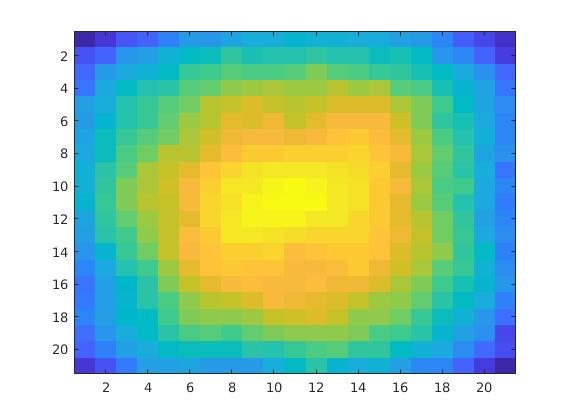
\includegraphics[width=1.3in]{pics/data_ent_squ_redo.jpg}}
\subfloat[]{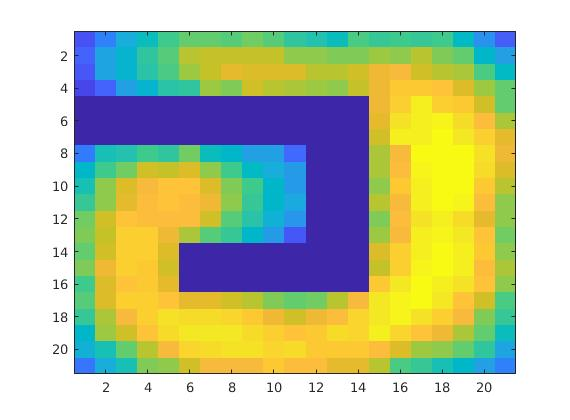
\includegraphics[width=1.3in]{pics/data_ent_obs_redo.jpg}}
\subfloat[]{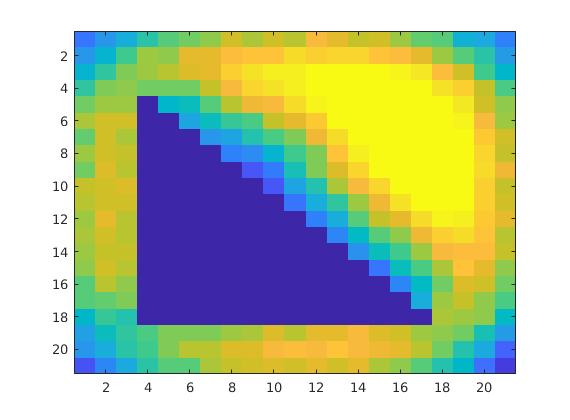
\includegraphics[width=1.3in]{pics/data_ent_tri_redo.jpg}}
\subfloat[]{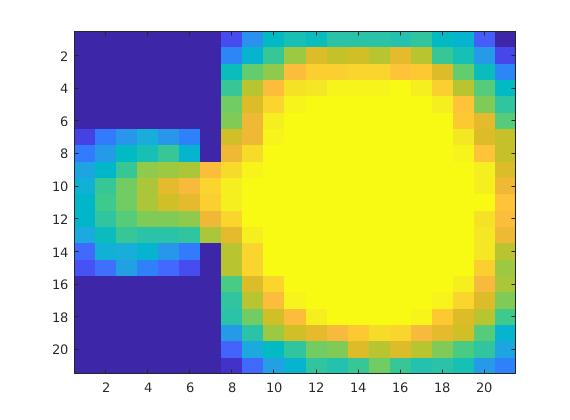
\includegraphics[width=1.3in]{pics/data_ent_tbc_redo.jpg}}
\caption{Value function of the various arenas for the agent aiming to purely maximise entropy. 
\textbf{(a)} is an empty arena. \textbf{(b)} is a snaking obstacle. \textbf{(c)} has a triangular obstacle with two corridors. \textbf{(d)} is an arena consisting of two rooms, where the agent initialises in the smaller room.\label{entfigs}
Here and in the following, agents were trained for $10^7$ episodes each of a length of 
twice the size of the environment with discount factor $\gamma=0.9$ and 
learning rate $\alpha=0.1$. 
For the single agent experiments the exploration rate was $\varepsilon=0.75$. 
	Yellow (blue) colour correspond to maximal (minimal) value at an 
arbitrary scale which is implied by the inverse RL scenario. 
	All values are non-negative. Inaccessible regions of the environment 
are assumed to have zero value.}
\end{figure}

Similarly in Fig.~\ref{entfigs}.\textbf{(d)}, the environment containing two different sized rooms, we observe that the greater values in the respective rooms are toward the centre, giving greater access to the remainder of the environment; however, as can be noted, the restricted region of the path between the two rooms also sees a greater valuation than other restricted regions, as this is the area that must be traversed to receive increased entropy.

This is consistent with what is observed in empowerment~\citep{klyubin2005empowerment}, particularly the cases of the mazes where an agent is in the state of greatest empowerment when it is not enclosed in walls, and over a defined $n$-step time horizon can actualise the greatest number of future states from the current state.

\subsubsection{Discounted empowerment\label{gammares_exp}}
When considering the case of quantities similar to entropy in our environment we considered the method we respectfully call $\gamma$-empowerment, accomplished by providing a negative reward for remaining in the same state between time steps.

As remaining in the same state between time steps is only possible in the case of colliding with an obstacle, and the high level of $\varepsilon$ makes this much more likely near corners or walls, we felt this was an appropriate quantity to consider in consort with entropy and empowerment, since under this scheme an agent should more highly value regions that provide future freedom of movement, and as opposed to the entropy case above, requires no calculation, and is easy to work with on-policy.

\begin{figure}[ht]

\centering
\subfloat[]{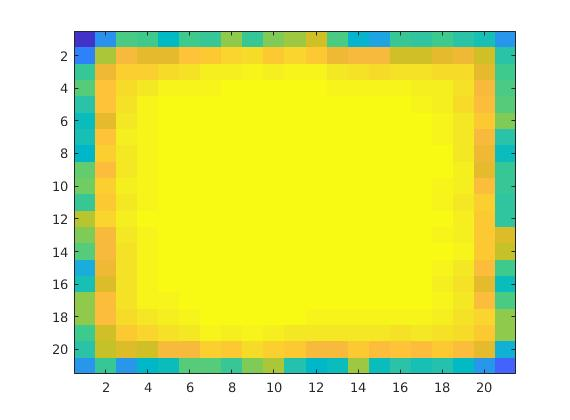
\includegraphics[width=1.3in]{pics/dat_gam_squ.jpg}}
\subfloat[]{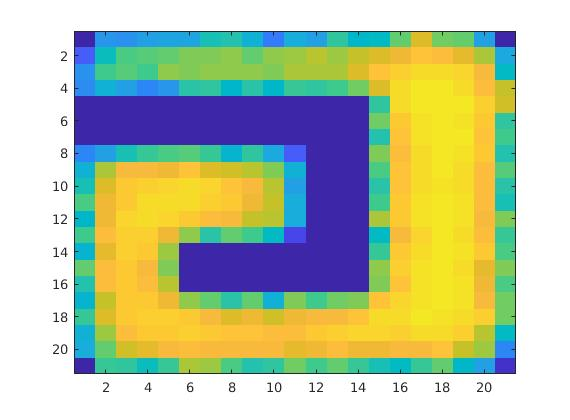
\includegraphics[width=1.3in]{pics/dat_gam_obs.jpg}}
\subfloat[]{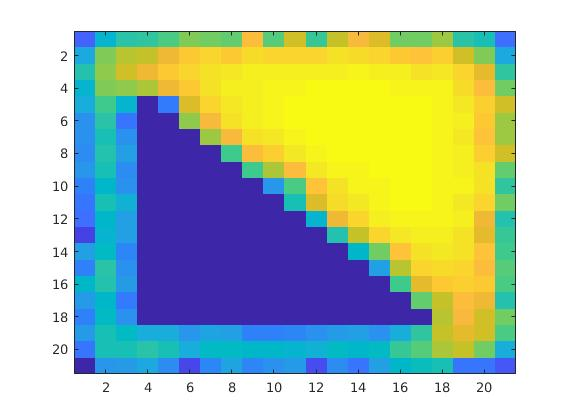
\includegraphics[width=1.3in]{pics/dat_gam_tri.jpg}}
\subfloat[]{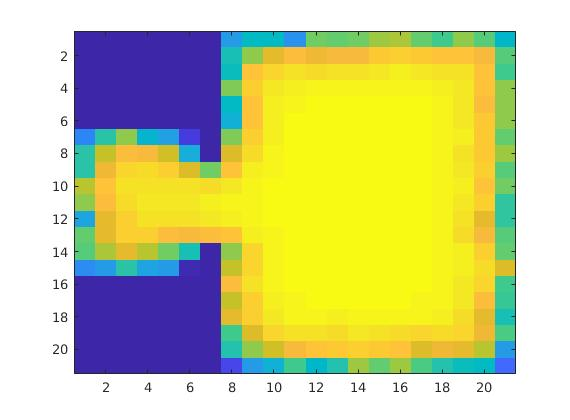
\includegraphics[width=1.3in]{pics/dat_gam_tbc.jpg}}
\caption{Value function when aiming to purely maximise $\gamma$-empowerment (\ref{eq:gamma_powerment}), with the obstacles, episodes, episode length and parameters as in Fig.~\ref{entfigs}\label{entsimilarfigs}}
\end{figure}

%\begin{figure*}[ht]
%\centering
%{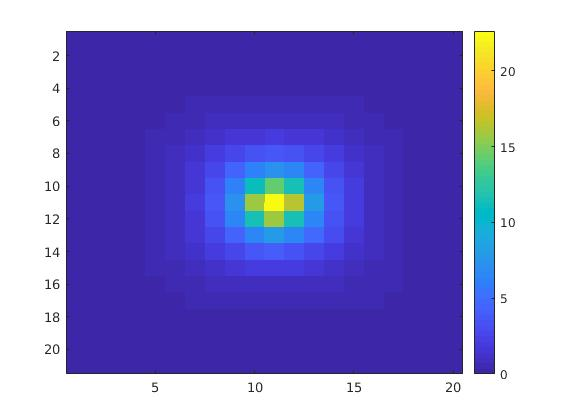
\includegraphics[width=1.3in]{pics/noobentsimilar.jpg}}
%{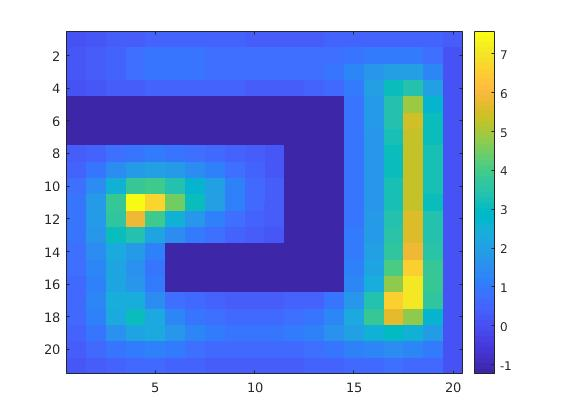
\includegraphics[width=1.3in]{pics/jobentsimilar.jpg}}
%{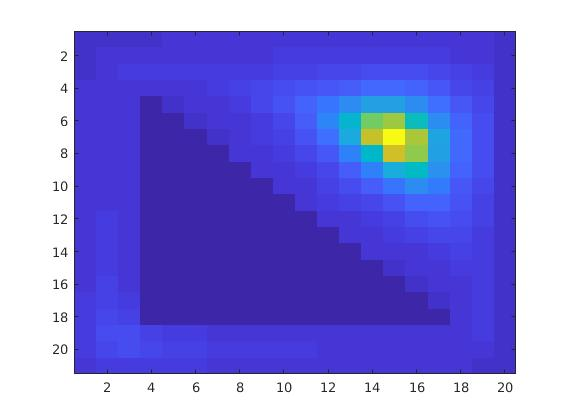
\includegraphics[width=1.3in]{pics/triobentsimilar.jpg}}
%{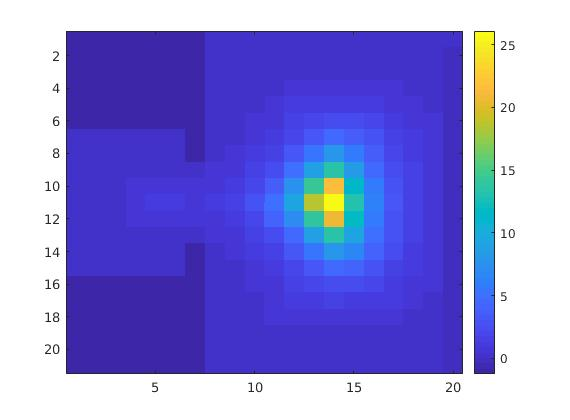
\includegraphics[width=1.3in]{pics/tbcentsimilar.jpg}}
%\caption{These colour maps represent the value of the various arenas the %agent was placed in when aiming to purely maximise entropy, with the %obstacles, episodes, episode length and parameters as in %Fig.~\ref{entfigs}}
%\label{entsimilarfigs}
%\end{figure*}

The resulting graphs can be seen in Fig.~\ref{entsimilarfigs}. Here we see similar regions of high valuation, with significantly increased value in the surrounding regions. This is consistent with what we would expect in an empowerment case, though with a substantially increased value for $n$ in the traditional case. 

We would not expect such a high value directly up to the wall regions, where in the maze variants seen in Klyubin et al.~\citep{klyubin2005empowerment} paper there is a smoother gradient between values, with much more distinct regions of increased entropy, closer to what we see in the entropy case.

\subsubsection{Flexibility of approach}
In this section we briefly touch on two other approaches we have used in experimentation to show that this approach is flexible in that it is not only applicable to entropy or entropy-like quantities over a state space. These are variants we have chosen to call \emph{prediction error reduction} and \emph{corner favouring}.

\begin{figure}[ht]
\centering
\subfloat[]{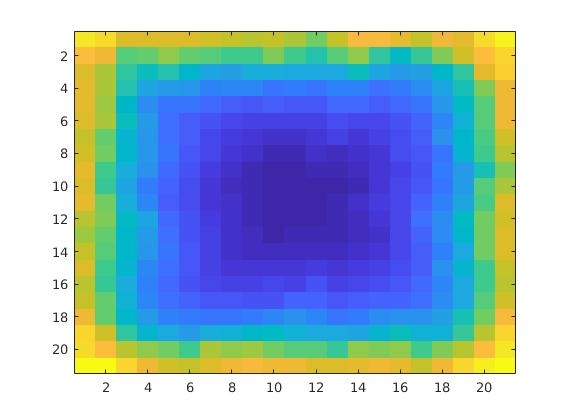
\includegraphics[width=1.3in]{pics/dat_wal_squ.jpg}}
\subfloat[]{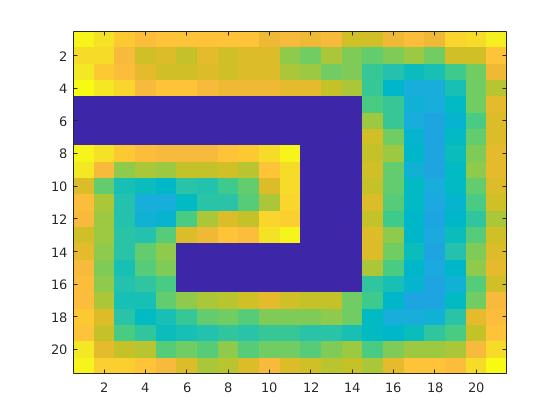
\includegraphics[width=1.3in]{pics/dat_wal_obs.jpg}}
\subfloat[]{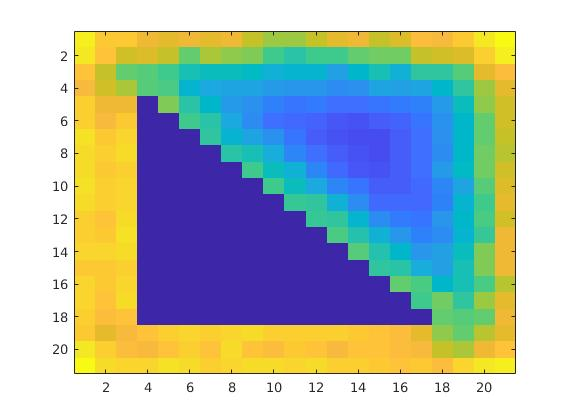
\includegraphics[width=1.3in]{pics/dat_wal_tri.jpg}}
\subfloat[]{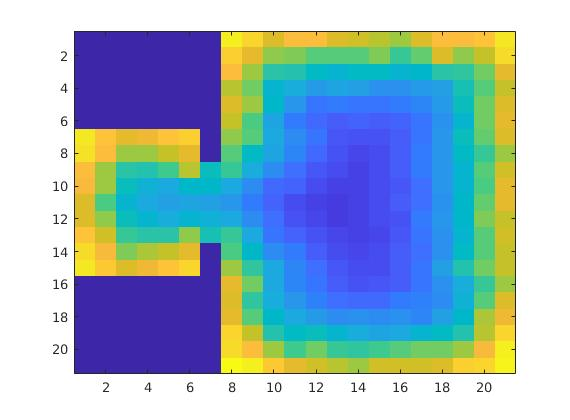
\includegraphics[width=1.3in]{pics/dat_wal_tbc.jpg}}\\
\subfloat[]{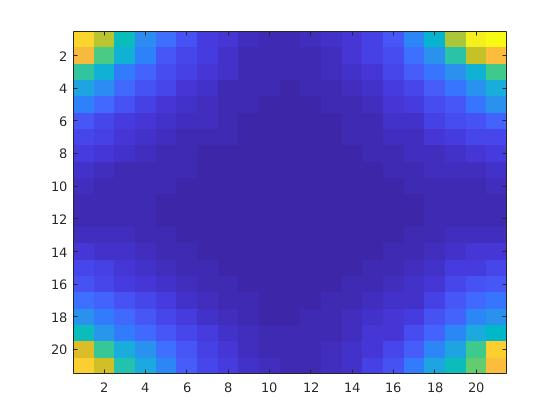
\includegraphics[width=1.3in]{pics/squ_cor.jpg}}
\subfloat[]{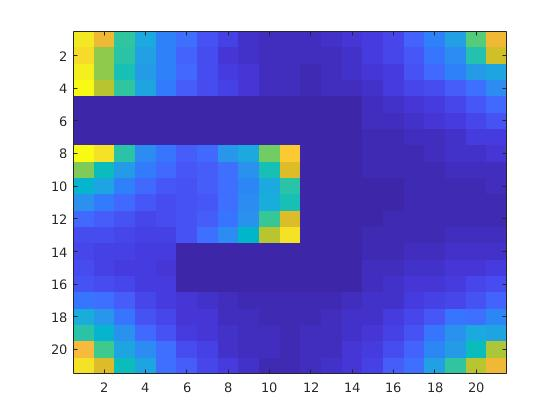
\includegraphics[width=1.3in]{pics/obs_cor.jpg}}
\subfloat[]{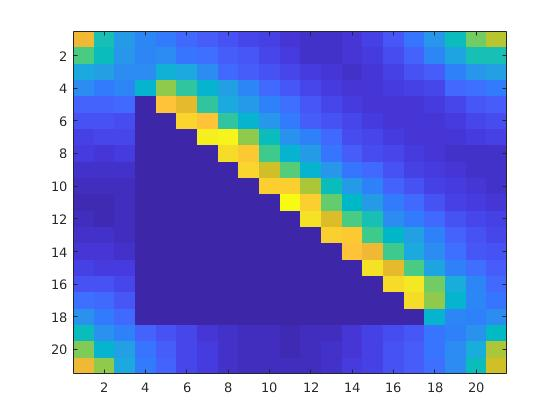
\includegraphics[width=1.3in]{pics/tri_cor.jpg}}
\subfloat[]{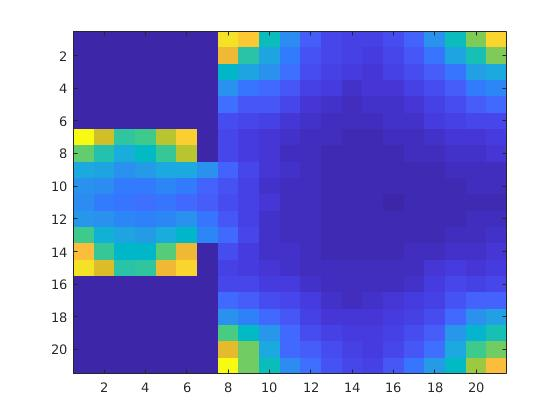
\includegraphics[width=1.3in]{pics/tbc_cor.jpg}}
\caption{Value function for an agent rewarded for obtaining sensory values of obstacles or walls in the environment, with the obstacles, episodes, episode length and parameters as in Fig.~\ref{entfigs}. Subfigures \textbf{(a)-(d)} represent the prediction error reduction variants, and the subfigures \textbf{(e)-(h)} represent the corner favouring variants.\label{othervariants}}
\end{figure}

Both sets of images seen in Fig.\ref{othervariants} use very simple reward schemes, only receiving rewards when they are located adjacent to walls and corners respectively. These types of regions are highly useful in noisy environments for localisation and reduction in prediction error, but in essence can serve an additional purpose in control schemes, that perhaps where there is no task relevant information, in a highly dynamic environment an agent should look to remove itself to these less task critical areas.

\subsection{Multi-agent RRL}
\label{sharedspace}
A natural extension of the basic RRL concept we have implemented so far is the extension to multi-agent systems, be they robot and human or multi robot tasks and environments. We are particularly interested in the concept of \emph{socially empowered} robots, given that we can expect that many tasks in logistic and exploratory domains will require robots to work in tandem, or indeed search in tandem for some task related information.

\begin{figure}[ht]
\centering
\subfloat[]{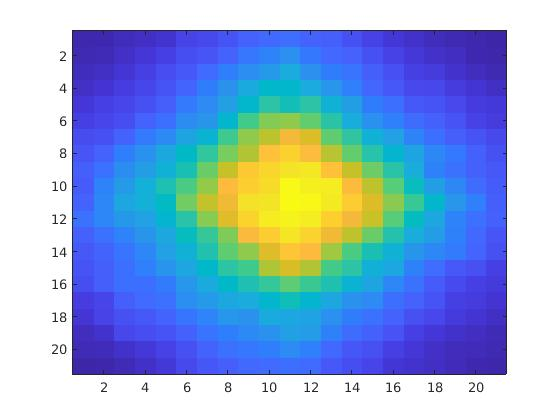
\includegraphics[width=1.3in]{pics/squ_social_emp.jpg}}
\subfloat[]{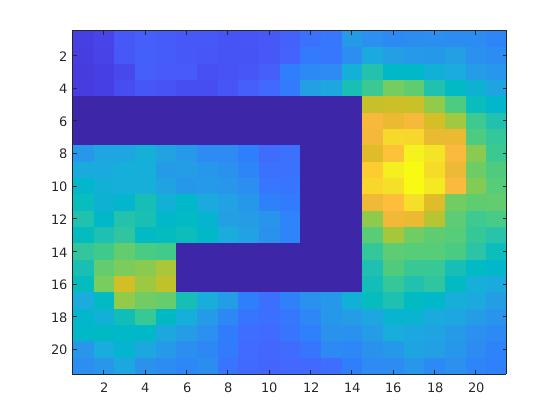
\includegraphics[width=1.3in]{pics/obs_social_emp.jpg}}
\subfloat[]{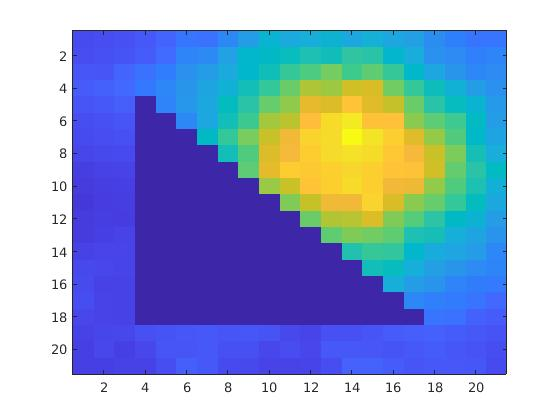
\includegraphics[width=1.3in]{pics/tri_social_emp.jpg}}
\subfloat[]{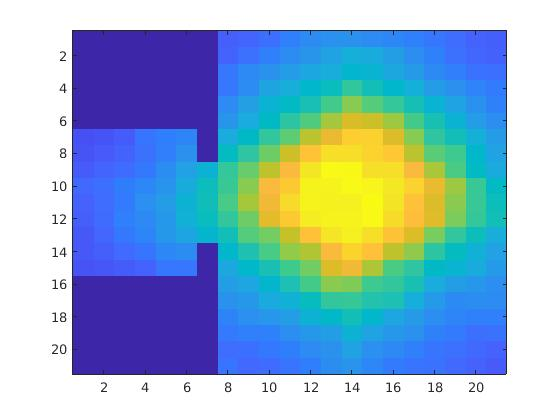
\includegraphics[width=1.3in]{pics/tbc_social_emp.jpg}}
	\caption{Value function for one of two agents rewarded for arriving in a nearby place to the other agent. Exploration rate is reduced: $\varepsilon = 0.50$ and other parameters are 
	as in Fig.~\ref{entfigs}.\label{social}. 
	Both agents share a state-action value function.}
\end{figure}

Reducing the $\varepsilon$ in the multi-agent system to $\varepsilon = 0.5$ seemed prudent, as the agents are attempting a mutual goal, and such a high level of exploration lead to too much noise to obtain anything reasonable; however, even this small reduction which still allows for significant exploration resulted in an interesting outcome, when rewarding the agents for being within a Manhattan distance of $5$ from one another.

What we see here is a high valuation of mutual space where joint activity is more likely, this has clear use cases in multi-agent tasks, where an agent perhaps moves to these high mutual value regions to recruit other agents where it has otherwise identified a task it is unable to complete alone.

\subsection{Remarks}
Rewarding an agent based on entropy leads to valuation of states which is commensurate with what one would expect in an empowerment approach, with the benefit that it can be computed on policy, without the necessity to exhaustively compute over all policies and time series.

Similarly, considering the easier to compute $\gamma$-empowerment, we are able to obtain a valuation similar to what we would expect from an empowerment approach; however, we observe that the valuation remains very similar over the open regions with no clear peak value in the environment, which may not prove as useful to the goal of intrinsic motivation over potentially dynamic environments as it shows a tendency to prefer vast regions in the state space, which will make isolating the most interesting or free regions over a complex or dynamic space much more unlikely.

We have also shown that the approach is flexible, highlighting regions such as walls and corners, regions that may be preferable in various existing control architectures. Additionally, we have shown that the approach is consistent in mulit-agent systems, and when rewarding agents for being in a proximity with other agents, what emerges is akin to the empowerment-like case, and should be viewed as a socially empowered state.

%%Where reduction in prediction error and relocalising are key priorities for a lost agent, we can also consider employing our variants in Sect.~\ref{prederr} and Sect.~\ref{cor} to move to regions outside of the state space, where there may be less task dependent information, yet the information is consistent and stable to relocalise and return to searching for task relevant information with a better understanding of where such information seen in the other variants can be found.

All of these variants here serve as a compliment to traditional reinforcement learning approaches through the use of the reflexive component, and indeed, can also be considered in tandem with one another. An intrinsically motivated, agent should seek out regions which are interesting or surprising as in Sect.~\ref{singlesect}, where no task relevant information is available in these identified regions of interest, the agent should return to regions where prediction error can be minimised, and relocalisation is possible, and the cycle should repeat, in a control system, perhaps after sufficient searching of the state space, the agent should move to regions which have minimal impact on a potentially dynamic environment, such as a corner, and wait to search again later.

Alternatively, we consider that if there is no task dependent information available, a continually learning agent should seek out these surprising regions, with the aim of learning more about the environment and correcting the model, by more accurately learning state transition probabilities, or learning about features present in these high interest subspaces, to better perform tasks in the future when this information becomes available.


\section{Discussion\label{Discussion}}

\subsection{Exploration vs.~exploitation}

The exploration-exploitation dilemma is not a solved problem in any of the various domains that it has been researched in. We presented here a use case for utilising entropy as a reward on its own or in conjunction with other rewards to highlight the best regions available to an agent in an environment where there is no clear goal. In doing so we have found that these regions which are considered highly valued are similar to those found in empowerment, where the agent more highly values regions from which it is able to access a larger subset of the state space over any given discrete time frame.

As opposed to having to create sophisticated models for task location, the use of entropy maximisation may enable agents to \emph{find} a task or location when lost in a changing environment. In future work we intend to consider the problem using actor-critic algorithms where the actor and critic with two different state-action value functions, and to employ this in a simulated dynamic environment, as well as employing this as a hierarchical model alongside other functions or goals to observe the possibility of robotic self motivation.

%\subsection{Markov property}


\subsection{Intrinsic motivation}
The search for an intrinsic motivation for an agent to perform any given task, develop new behaviours, or learn its own embodiment is and take advantage of that is a key task in the development of continually learning, adaptable agents which are capable of working in highly dynamic environments. It is essential that an agent is able to identify important or interesting regions in the sensorimotor space, both to learn the model, or in fact learn a goal where no clear goal is immediately visible. 

Empowerment seeks to do this~\citep{salge2014empowerment} by defining an empirical measure which can be performed over the state-action space to definitively state the best possible states for an agent to be in to have sufficient future degrees of freedom. This valuable concept is unfortunately subject to the curse of dimensionality, and as such, other approaches to estimating empowerment have been sought~\citep{zhao2019learning}. We believe that we have shown that entropy maximisation allows for an agent to approximate such a position utilising an on-policy approach over varying environments, by instead considering more interesting or surprising regions of the state space to be the most valuable.

This can more concisely be thought of as a form of information empowerment, where, as opposed to the mantra ``All else being equal, be empowered''~\citep{klyubin2005all}, we consider that perhaps the notion in a adaptive learning agent should be ``all else being equal, be interesting''.

%\subsection{Local and global learning}

%Additionally, extending beyond known environments, we consider, as mentioned in Sect.~\ref{prederr}, we consider the approach may be a natural extension to SLAM architectures, when an agent is performing traditional SLAM functions, the agent will take not of interesting regions, perhaps where sensor readings provide reduced or noisy feedback, to return to in future with high priority, in doing so reducing the error whilst providing more immediate exploitation centric functionality.

\section{Conclusion}

Reflexive reinforcement learning (RRL) is a new direction in machine learning. It is based on the observation that in learning problem where no direct gradient can be used in order to adapt to a particular, the representation of information from the environment (such as state information or evaluative information) requires not only guiding principles (such as smoothness, consistency and locality), but also provides information that can be used to decide about the actions of an agent.

The advantage of reflexive reinforcement learning is that an agent can learn 
even in the absence of an evaluative signal (reward and punishment), it can 
bootstrap elementary actions (as in homeokinesis~\citep{der2012playful}) or can learn about options in the environment (as in empowerment~\citep{klyubin2005empowerment}),
and obtain more meaningful and generalisable 
representations (see~\citep{smith2018evaluation}).

The unavoidable difficulty in reflexive reinforcement learning consists in the 
fact that the use of quantities that are eventually based on the reward as a
reward, introduces a feedback loop which can lead to instabilities or divergences. This is not unknown in RL, where e.g.~an often visited source of low reward can dominate a better source of reward that is rarely found, or in cases where correlations among basis functions lead to divergences as notice already in Ref.~\citep{baird1995residual}. 

In reflexive reinforcement learning such 
feedback is even more typical, but can also be used to introduce structure the 
state space by self-organised pattern formation or to identify hierarchical 
relationships as will be studied in future. In order to keep the effects of 
self-referentiality under control and to make use of their potential
a dynamical systems theory of reinforcement learning is required that 
does not only consider the agent as a dynamical system, but the full interactive 
system formed by the agent, its environment and its internal representations.

Finally, we should stress the importance of the presented concept of RRL for explainable AI and its relation to information processing in the brain.

\section*{Broader Impact}

\emph{Reflexive reinformcement learning}
has a variety of potential applications in terms of control architecture for autonomous agents, as well as less lofty pursuits. 
As shown in Fig.~\ref{entfigs} and Fig.~\ref{entsimilarfigs}, the agent identifies the 
highlighted regions as a preferrence to avoid walls and obstructions as these in the presence of
noise may to lead to behaviour that remains unexplainable to ab observer. Likewise, \emph{empowerment} gives the agent a chance to produce controllable and predictable behaviour under these conditions. Although we have outlined here merely its basics,  RRL opens a new avenue to responsible and safer robotic behaviour and presents an agent with capabilties analogous to introspection, self-exploration, and self-optimisation that will be highly beneficial in autonomous robotics and 
human-robot interaction.
%We believe there is potential here to consider the notion of \emph{curiosity path planning}, where an agent plans the route on the basis of interesting regions within a known environment to better learn about, or be available for future tasks.

%\section*{Acknowledgements}

%\noindent t.b.a.
%This research was funded by EPSRC through the CDT RAS at Edinburgh Centre for Robotics. Discussions with Calum Imrie and Simon Smith are gratefully acknowledged.

\bibliographystyle{plainnat.bst}
\bibliography{bib_file}

\section*{Supplementary material}
\begin{itemize}
	\item Generalisation to continuous state and action spaces
	\item Additional multi agent figures and variants
\end{itemize}

\end{document}